\documentclass[a4paper]{article}
% Start Preamble
\usepackage[utf8]{inputenc}
\usepackage{fullpage}
\usepackage[english]{babel}
\usepackage{color}
\usepackage{url}
\usepackage{standalone}
\usepackage{parskip} % Package to tweak paragraph skipping
\usepackage{hyperref}
\usepackage{amsmath,amssymb}
\usepackage{color}
\usepackage[version=4]{mhchem} 
\usepackage{bm}
\usepackage{verbatim}
\usepackage{subfig}

\title{Reflection and Refraction}
\author{Lauren Shriver}
\date{September 26 2018}

\begin{document}
\maketitle

\section*{Specular and Diffuse Relection}
There are two types of reflection: specular reflection and diffuse reflection. 
\subsection*{Aside}
First, we need to specify two "types" of light rays
\begin{enumerate}
    \item \textbf{Incidence ray} = a light ray approaching a reflective surface
        \begin{itemize}
            \item The \textbf{angle of incidence} $\theta_i$ is the angle of the incidence ray with respect to the axis perpendicualr to the reflective surface 
        \end{itemize}
    \item \textbf{Reflective ray} = a light ray that "bounces" off the reflective surface once the incidence ray collides with the surface 
\end{enumerate}
\begin{figure}[htp!]
        \centering
        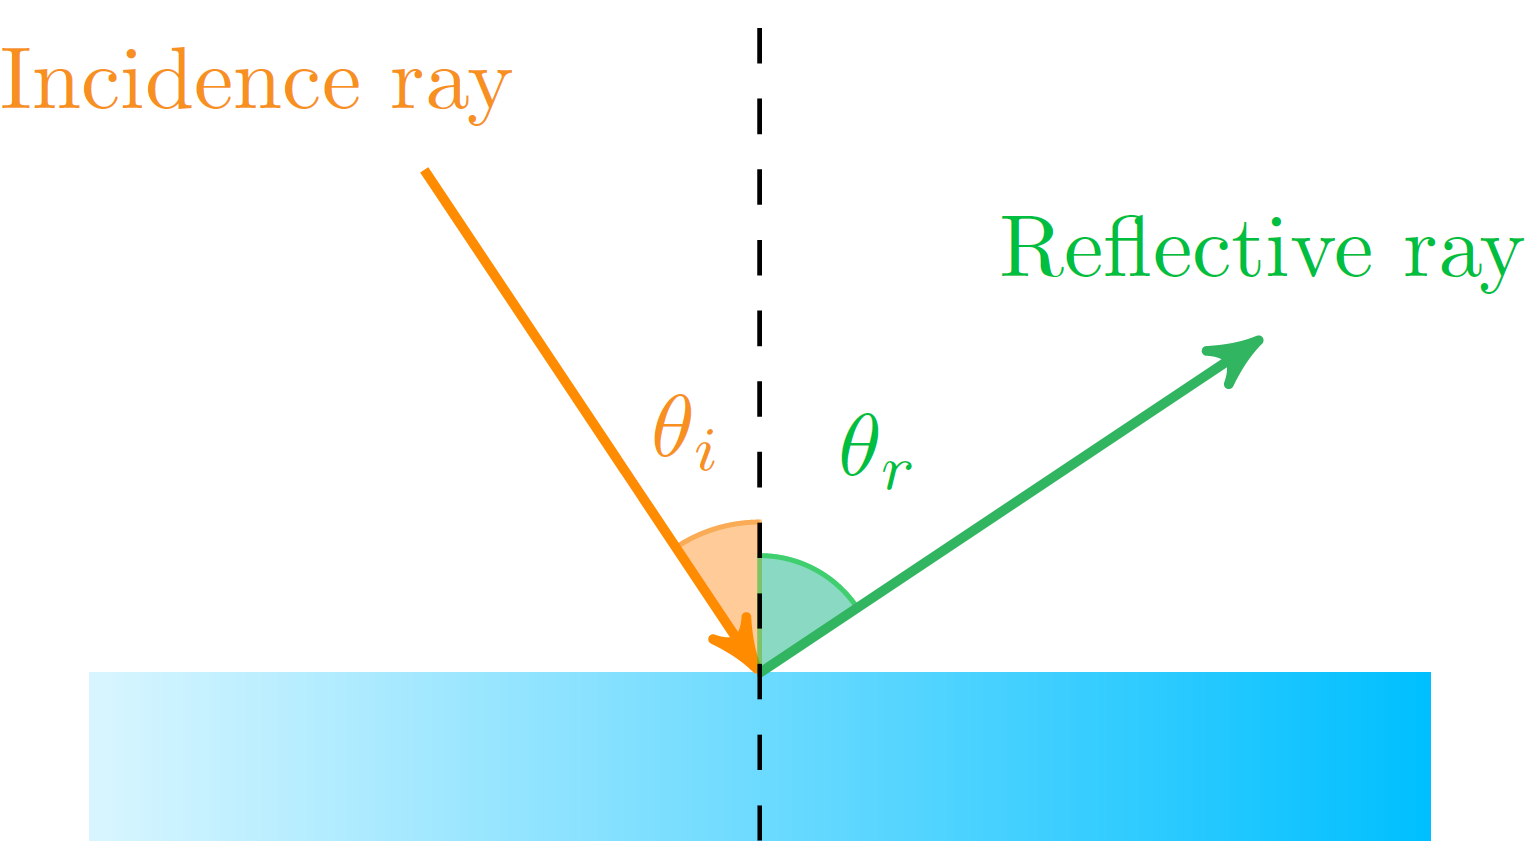
\includegraphics[width=7cm]{incidence_refractive.png}
        \caption{An incidence ray (orange) and its corresponding reflective ray (green). $\theta_i$ denotes the angle of incidence and $\theta_r$ denotes the angle of reflection.}
        \label{fig:my_label}
\end{figure}
\subsection*{Specular Reflection}
The defining property of \textbf{specular reflection} is $\theta_i = \theta_r$ 
\section*{Relection vs. Refraction}
\end{document}
